
During the dedicated experiment that took place in the SPS
in 2018 with the CCs, the measured emittance
growth was found to be a factor four (on average) lower than
expected from the theory (see Section~\ref{sec:meas_2018_vs_theory}). The reason for this discrepancy remained unresolved for some time, as detailed follow-up studies (see Chapter~\ref{Ch:investigating_discrepancy}) investigated and excluded a number of possible explanations for the discrepancy.
It was recently found, that the beam transverse impedance, which is not included in the theory~\cite{PhysRevSTAB.18.101001} used for the comparison with the measurements may impact the noise-induced emittance growth and explain the experimental observations. Here, the damping mechanism from the beam transverse impedance is investigated and discussed with detailed PyHEADTAIL simulations.

The structure of this chapter is as follows:




\section{SPS transverse impedance model}
The PyHEADTAIL studies presented in this chapter are performed including the detailed transverse impedance model of the SPS machine~\cite{sps_impedance_model_git}. This model has been developed through a combination of theoretical computations, electromagentic simulations and was benchmarked with beam-based measurements~\cite{Salvant:1274254, Zannini:1561199, Salvant:1271349, Zannini:2141779}. 
It includes the contributions from all the individual elements in the SPS lattice i.e. the resistive wall, the indirect space charge, the kickers, the RF cavities (200\,MHz and 800\,MHz), the step transitions and the horizontal and vertical beam position monitors~\cite{Zannini:2141779}. 
%https://indico.cern.ch/event/299470/contributions/686509/attachments/564150/777102/LIUSPS_transverse_imp_5.pdf
% The Wall contribution included both the resistive wall and the indirect SC.
The transverese imepedance of SPS is displayed in Fig. The dipolar and quadrupolar components are plotted seperately.


\begin{figure}[!ht]
    \centering
    \begin{subfigure}[t]{0.45\textwidth}
        \centering
        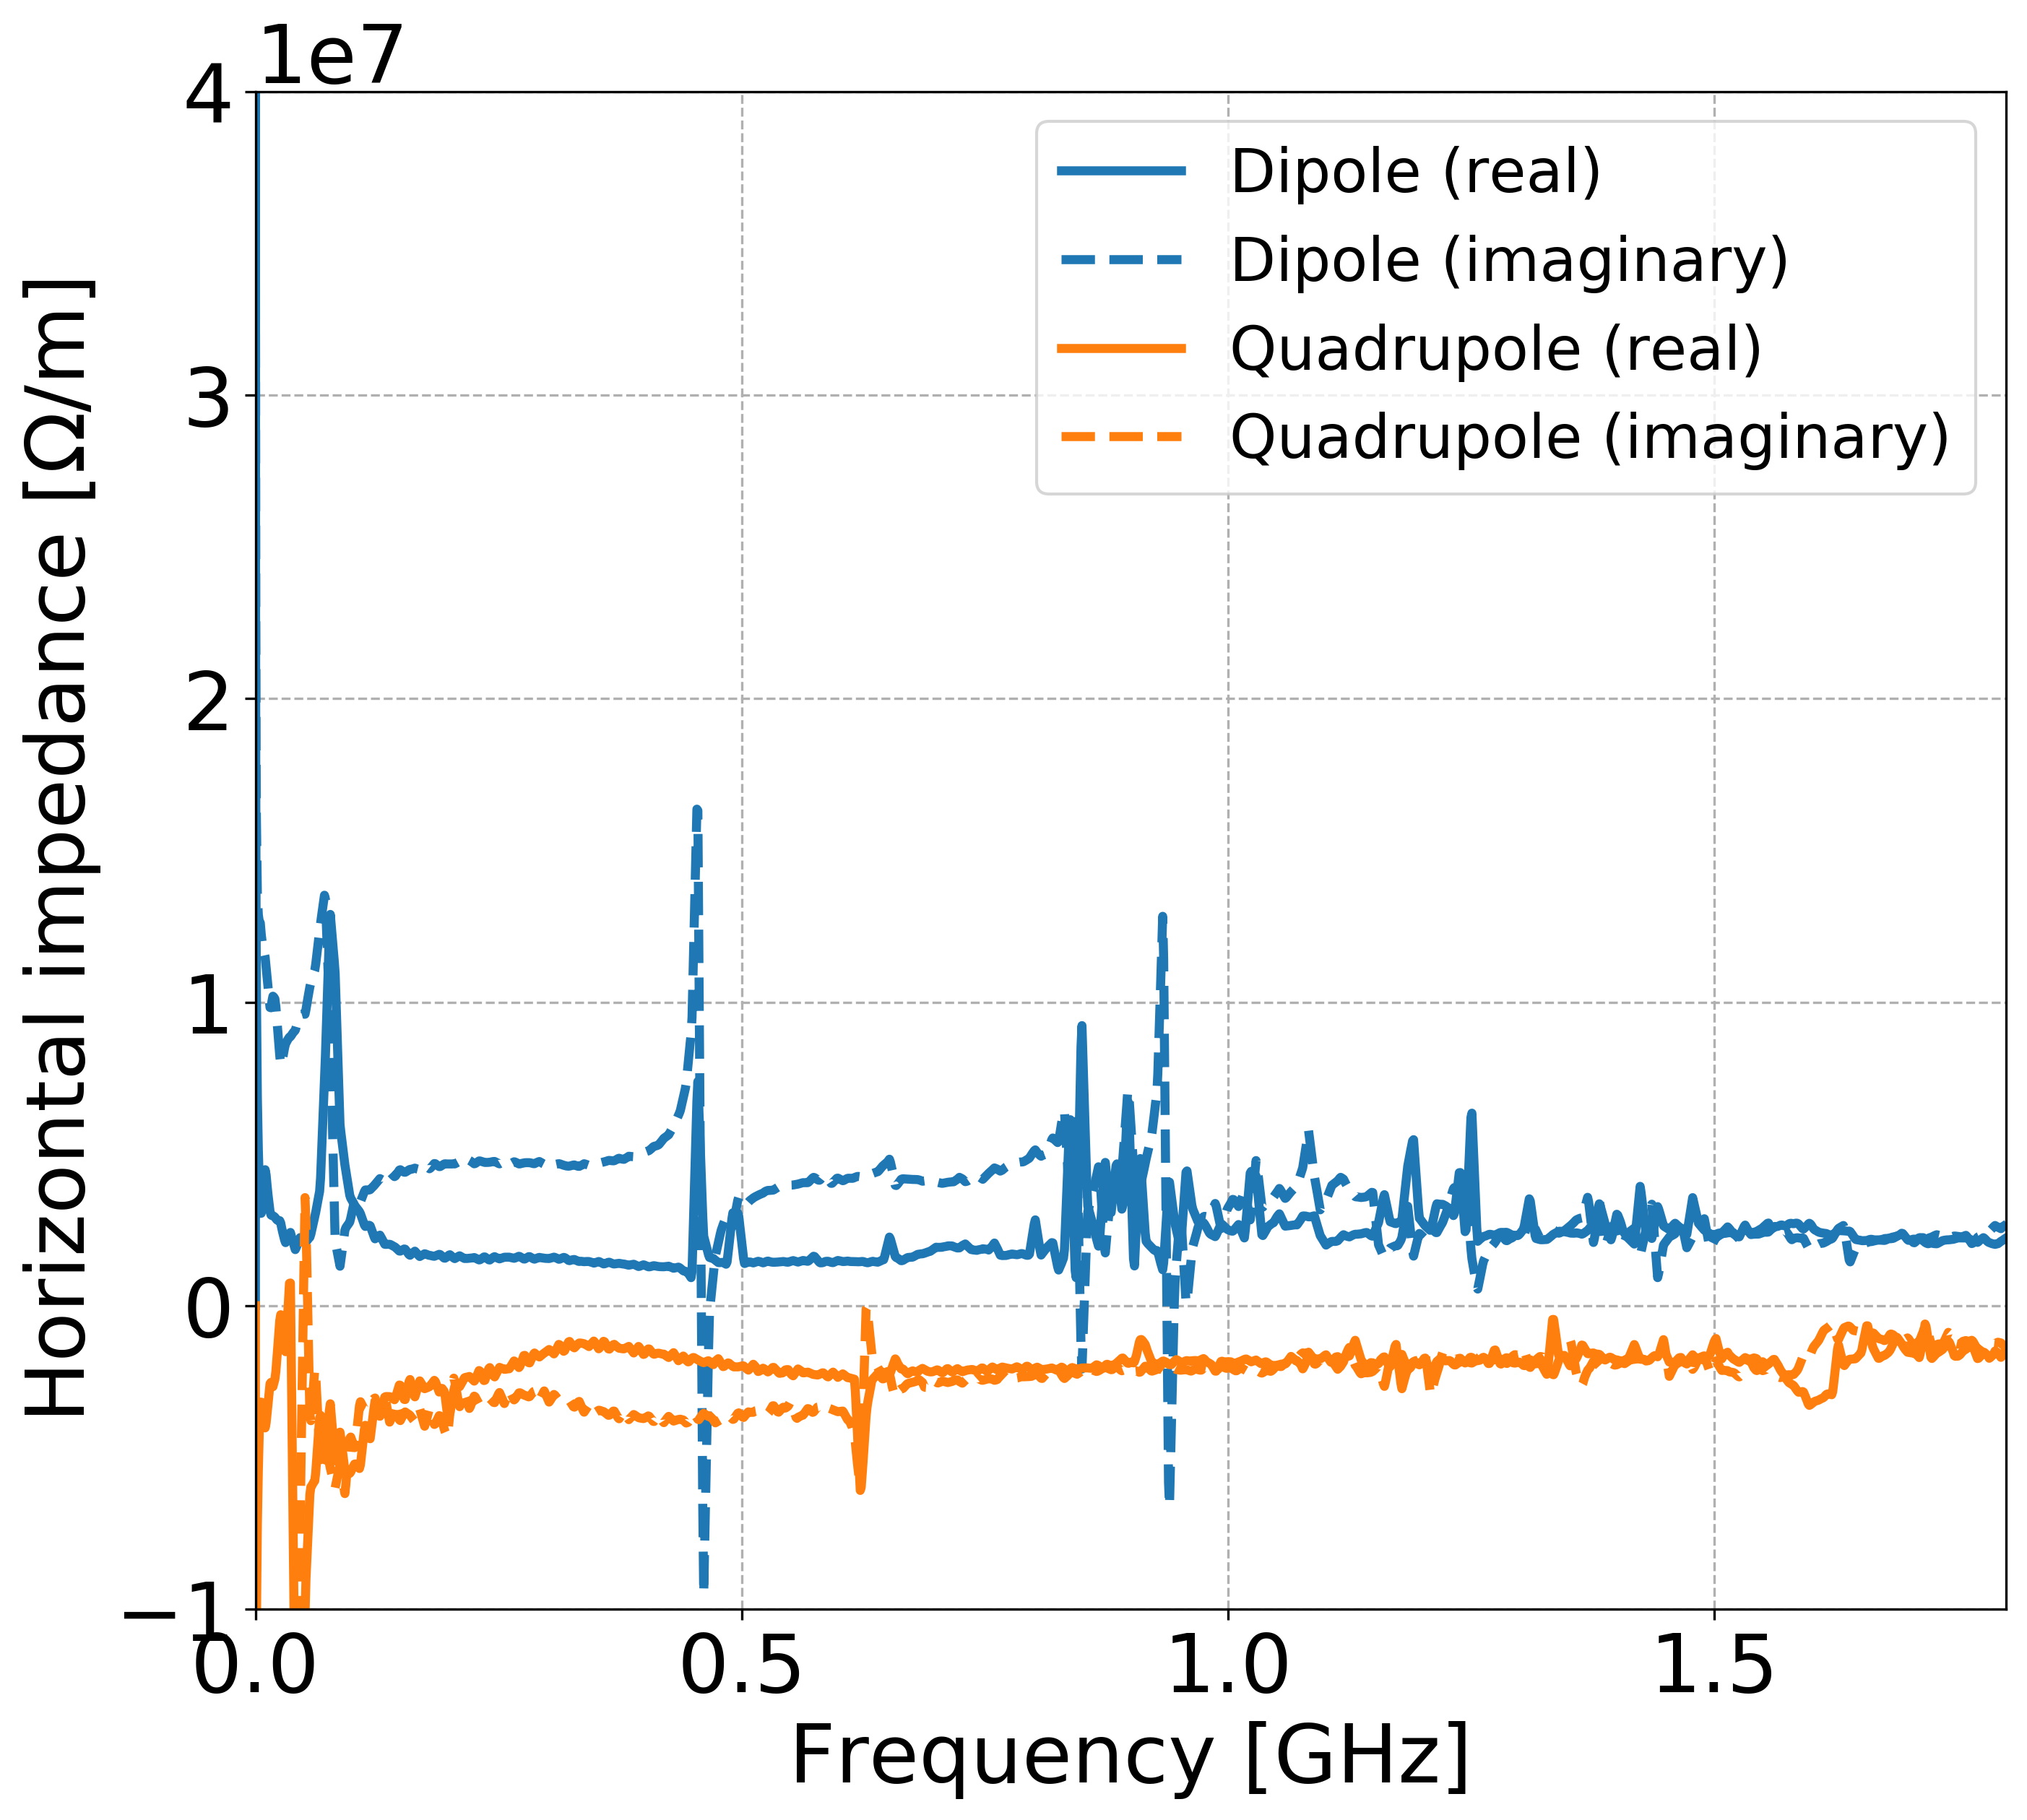
\includegraphics[width=1\textwidth]{images/Ch7/Q26_complete_SPS_model_impedance_H_plane.png}
        %\caption{$y=\sin(2 \pi f t),\ f=50$ Hz}
        %\label{fig:add_label_here}
    \end{subfigure}
    \hfill
    \begin{subfigure}[t]{0.45\textwidth}
        \centering
        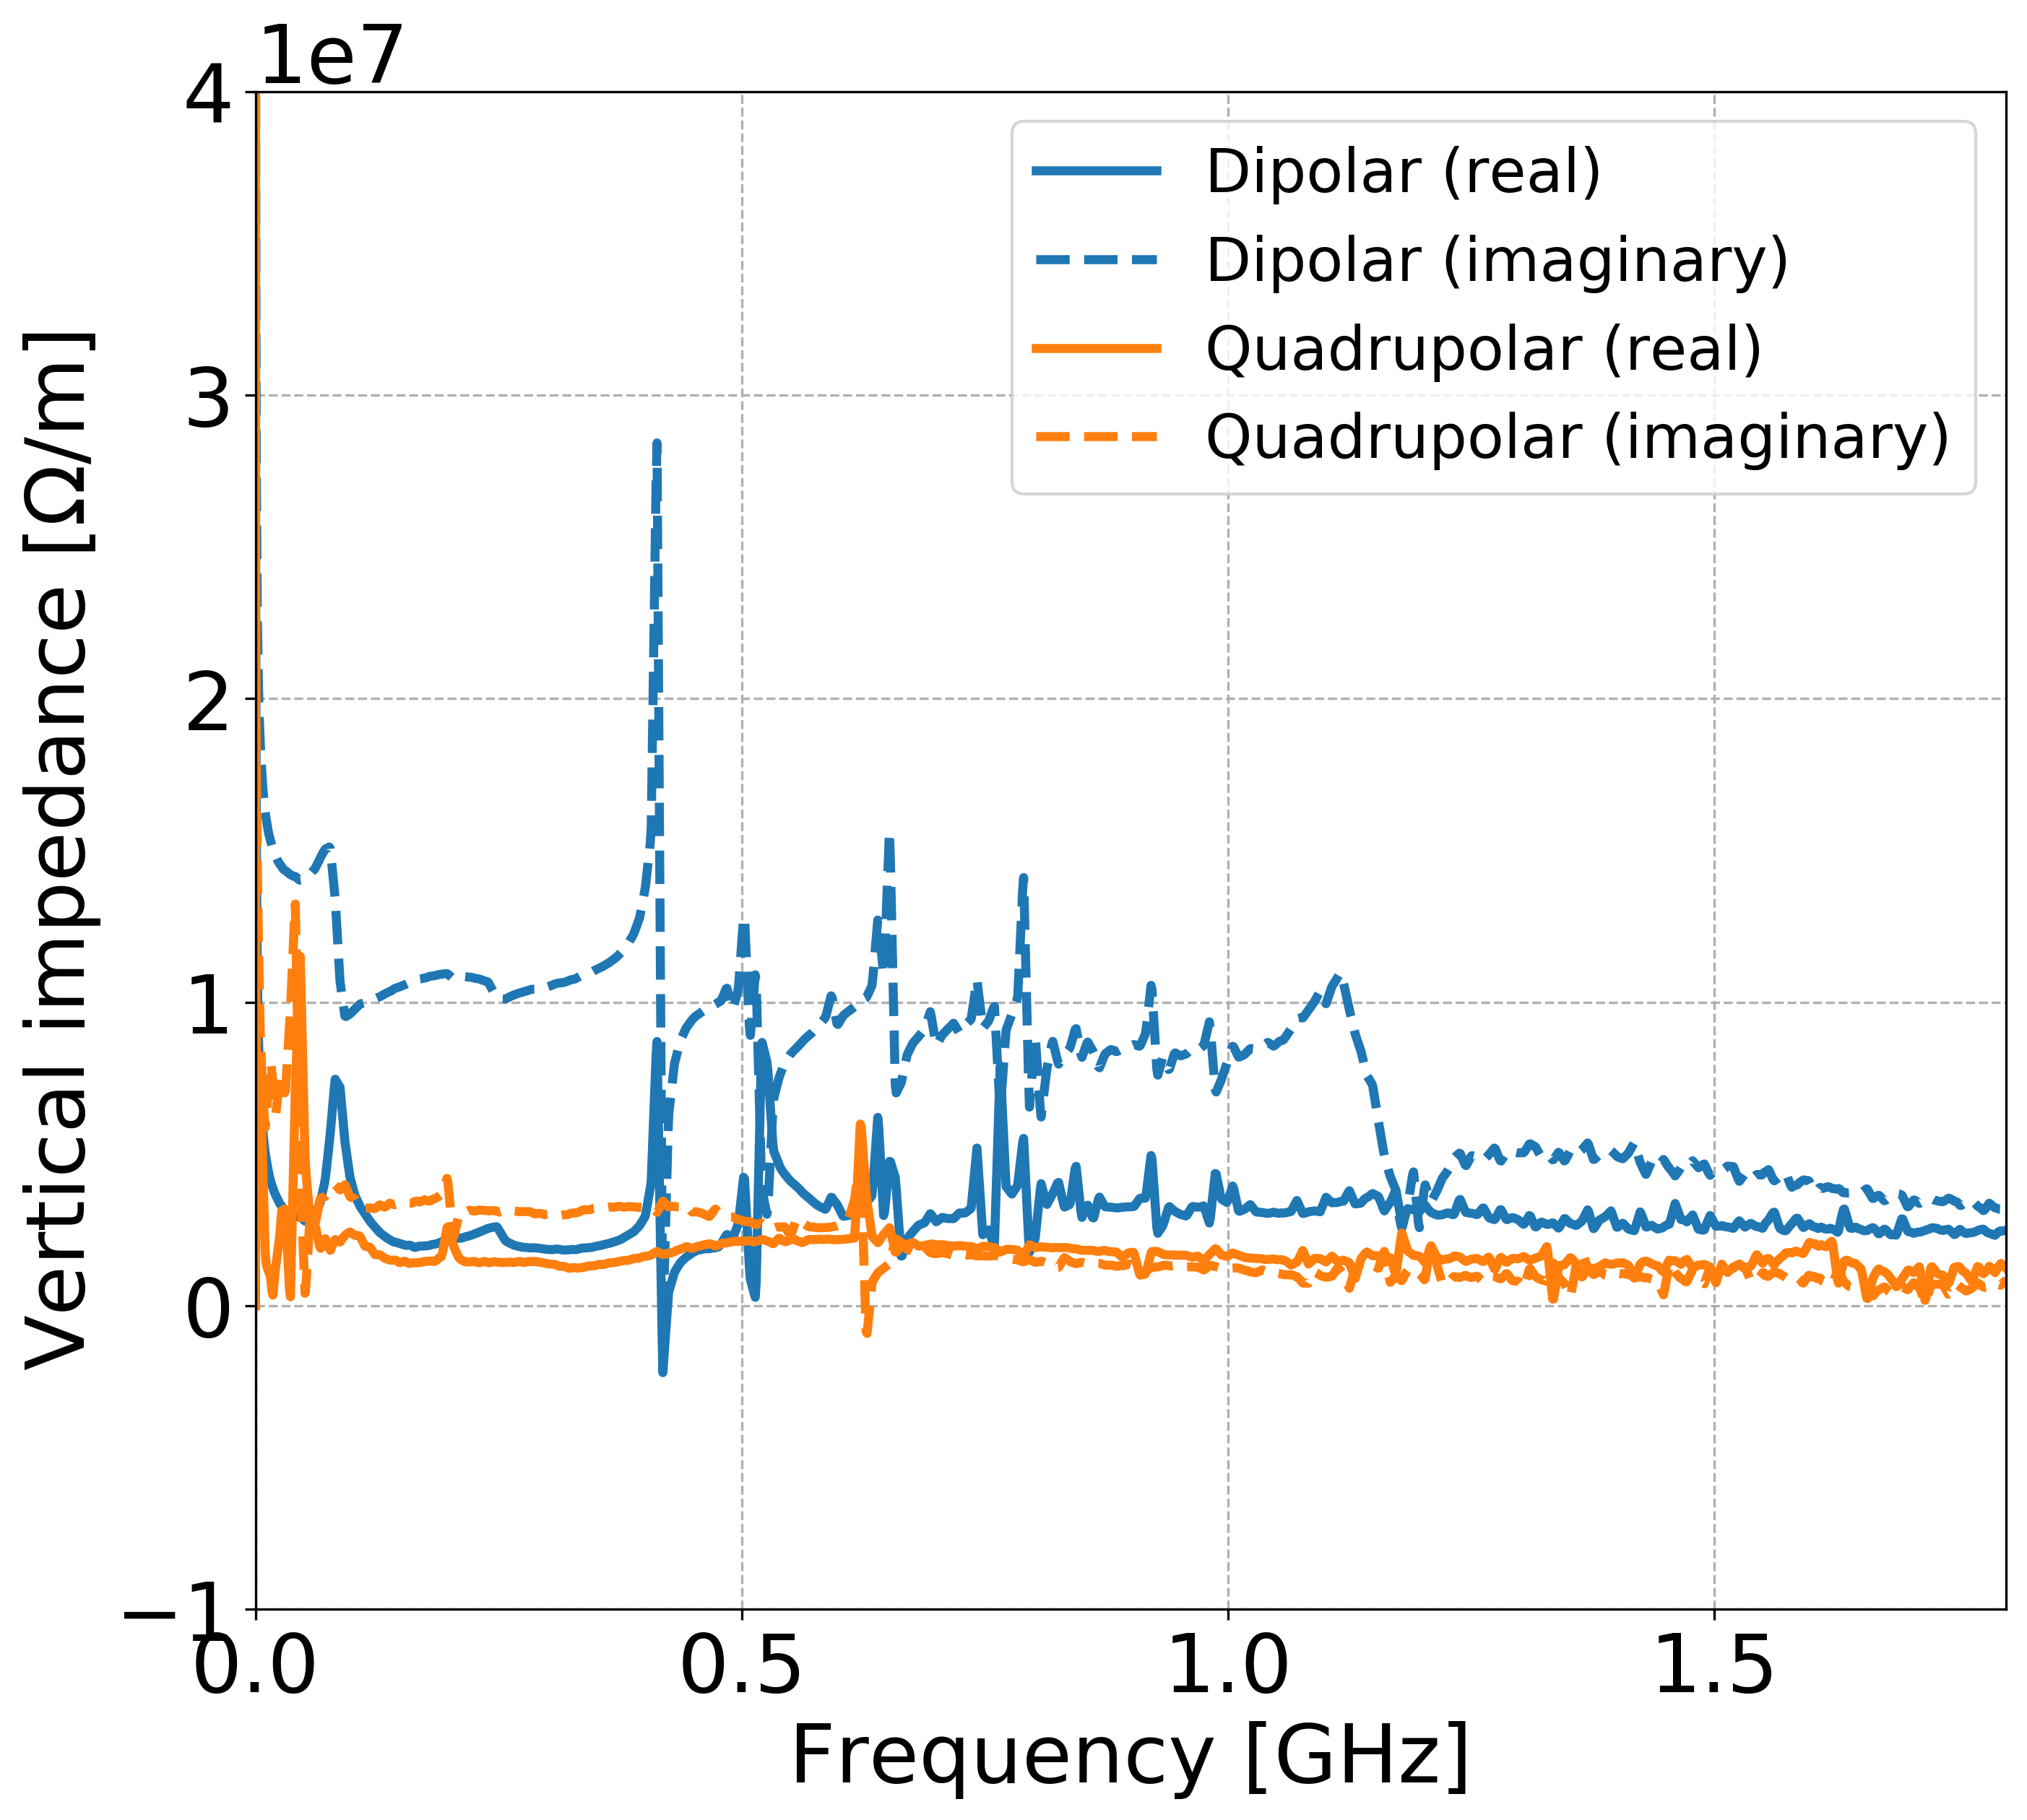
\includegraphics[width=1\textwidth]{images/Ch7/Q26_complete_SPS_model_impedance_V_plane.png}
        %\caption{Discrete Fourier transform}
        %\label{fig:add_label_here}
    \end{subfigure}
    \hfill
     \caption{Horizontal (left) and vertical (right) impedance model of the SPS.} % bunch passage
     \label{fig:sps_impedance_model_H_V}
 \end{figure}



\section{Simulations setup}




\section{First observations of emittance growth suppression from impedance}